\documentclass[
 size=12pt,
 paper=smartboard, %a4paper, smartboard, screen
 mode=present, %present, handout, print
 display=slides, % slidesnotes, notes, slides
 style=tuliplab,  % TULIP Lab style
 pauseslide,
 fleqn,leqno,clock]{powerdot}

\usepackage{amssymb}
\usepackage{amsmath}
\usepackage{rotating}
\usepackage{graphicx}
\usepackage{boxedminipage}
\usepackage{media9}
\usepackage{rotate}
\usepackage{calc}
\usepackage[absolute]{textpos}
\usepackage{psfrag,overpic}
\usepackage{fouriernc}
\usepackage{pstricks,pst-node,pst-text,pst-3d,pst-grad}
\usepackage{moreverb,epsfig,color,subfigure}
\usepackage{color}
\usepackage{pstricks}
\usepackage{pstricks-add}
\usepackage{pst-text}
\usepackage{pst-node, pst-tree}
\usepackage{booktabs}
\usepackage{etex}
\usepackage{breqn}
\usepackage{multirow}
% \usepackage{pst-rel-points}
\usepackage{listings}
\usepackage{hyperref}
\hypersetup{ % TODO: PDF meta Data
  pdftitle={Presentation Title},
  pdfauthor={Gang Li},
  pdfpagemode={FullScreen},
  pdfborder={0 0 0}
}


% \usepackage{auto-pst-pdf}
% package to show source code

\definecolor{LightGray}{rgb}{0.9,0.9,0.9}
\newlength{\pixel}\setlength\pixel{0.000714285714\slidewidth}
\setlength{\TPHorizModule}{\slidewidth}
\setlength{\TPVertModule}{\slideheight}
\newcommand\highlight[1]{\fbox{#1}}
\newcommand\icite[1]{{\footnotesize [#1]}}

\newcommand\twotonebox[2]{\fcolorbox{pdcolor2}{pdcolor2}{#1\vphantom{#2}}\fcolorbox{pdcolor2}{white}{#2\vphantom{#1}}}
\newcommand\twotoneboxo[2]{\fcolorbox{pdcolor2}{pdcolor2}{#1}\fcolorbox{pdcolor2}{white}{#2}}
\newcommand\vpspace[1]{\vphantom{\vspace{#1}}}
\newcommand\hpspace[1]{\hphantom{\hspace{#1}}}
\newcommand\COMMENT[1]{}

\newcommand\placepos[3]{\hbox to\z@{\kern#1
        \raisebox{-#2}[\z@][\z@]{#3}\hss}\ignorespaces}


%%%%%%%%%%%%%%%%%%%%%%%%%%%%%%%%%%%%%%%%%%%%%%%%%%%%%%%%%%%%%%%%%%%%%%%%%%
%%% title
%%% TODO: Customize to your Own Title, Name, Address
%%%
\title{FLIP(00) Final-term Presentation}
\author{Rongxin Xu\\
Hunan University
% \href{mailto:gangli@acm.org}{gangli@acm.org}
% \and % more authors
}
\date{29 November 2019}



% Customize the setting of slides
\pdsetup{
% TODO: Customize the left footer, and right footer
rf={\copyright \emph{FLIP(00)}},
cf={FLIP(00) Presentation },
}


% Starts the document
\begin{document}

\maketitle

%%==========================================================================================
%%
\begin{slide}[toc=,bm=]{Outline}
	\tableofcontents[content=sections]
\end{slide}
%%
%%==========================================================================================

\section{Problem Statement}

\begin{slide}{Problem Description}
	\begin{center}
		\twotonebox{\rotatebox{90}{Defn}}{\parbox{.96\textwidth}
			{
				This is a problem with time-series prediction.
				After a month of making scientific observations
				and taking careful measurements,
				can predict total sales for every product and store in the next
				month.
				The raw dataset contains  train set with 2935849
				samples and 214200 unlabeled samples as test set.
				Through the train data, predict total sales for every
				product and
				store in the next month.}}
	\end{center}
\end{slide}

\begin{slide}{Data Set}
	\begin{center}
		\twotonebox{\rotatebox{90}{Defn}}{\parbox{.96\textwidth}
			{There are 6 data sets with a total of 11 attributes,
				the fllowings are the
				name and meaning of attributes.
			}}
	\end{center}
	\begin{center}
		\begin{itemize}
			\item Data List
		\end{itemize}
		\begin{description}
			\item[id]  an Id that represents a (Shop, Item) tuple within the
			      test set.
			\item[shop\_id] unique identifier of a shop.
			\item[item\_id] unique identifier of a product.
			\item[item\_category\_id] unique identifier of item category.
			\item[item\_cnt\_day] percentage of soul in the creature.
			\item[item\_price] current price of an item.
			\item[date] date in format dd/mm/yyyy.
			\item[date\_block\_num] unique identifier of item category.
			\item[item\_name] name of item.
			\item[shop\_name] name of shop.
			\item[item\_category\_name] name of item category.
		\end{description}
	\end{center}
\end{slide}

\section{Exploratory Data Analysis}
%
\begin{slide}{Data Information}
	\begin{center}
		The following 	is the statistical
		result of each attribute in sales\_train.csv.
		There are 6 numerical variables,
		and no missing values.
		The data is very clean and complete, So let's start visual
		analysis.
	\end{center}
	\begin{tabular}{ccccccc}
		\hline
		% after \\: \hline or \cline{col1-col2} \cline{col3-col4} ...
		        & date\_block\_num & shop\_id & item\_id & item\_price &
		item\_cnt\_day
		        &
		item\_category\_id
		\\
		\hline
		count   & 2935849          & 2935849  & 2935849  & 2935849     &
		2935849 & 2935849                                                \\
		mean    & 14.57            & 33       & 10197.23 & 890.62      &
		1.24    & 40                                                     \\
		std     & 9.42             & 16.23    & 6324.3   & 1726.44     &
		2.62    & 17.1                                                   \\
		min     & 0                & 0        & 0        & -1          &
		-22     & 0                                                      \\
		25\%    & 7                & 22       & 4476     & 249         &
		1       & 28                                                     \\
		50\%    & 14               & 31       & 9343     & 399         &
		1       & 40                                                     \\
		75\%    & 23               & 47       & 15684    & 999         &
		1       & 55                                                     \\
		max     & 33               & 59       & 22169    & 307980      &
		2169    & 83                                                     \\
		\hline
		%\bottomrule
	\end{tabular}
\end{slide}

\begin{slide}{Data Visualization}
	\begin{center}
		\twotonebox{\rotatebox{90}{Exp}}{\parbox{.96\textwidth}
			{Use EDA to plot the distribution of the data,
				can observate the data intuitively and
				find the relation between the attribute values.
			}}
	\end{center}
	\begin{center}
		\begin{itemize}
			\item Figures
			      \begin{itemize}
				      \item Histogrm
				      \item Boxplot
				      \item Scatterplot Plot
				      \item Correllogram
			      \end{itemize}
		\end{itemize}
	\end{center}
\end{slide}

\begin{slide}{Data Visualization}
	\begin{center}
		\twotonebox{\rotatebox{90}{Exp}}{\parbox{.96\textwidth}
			{It seems that item\_id and
				shop\_id has a huge impact on sales and sales tend to decline
				with the date.
			}}
	\end{center}

	\begin{center}
		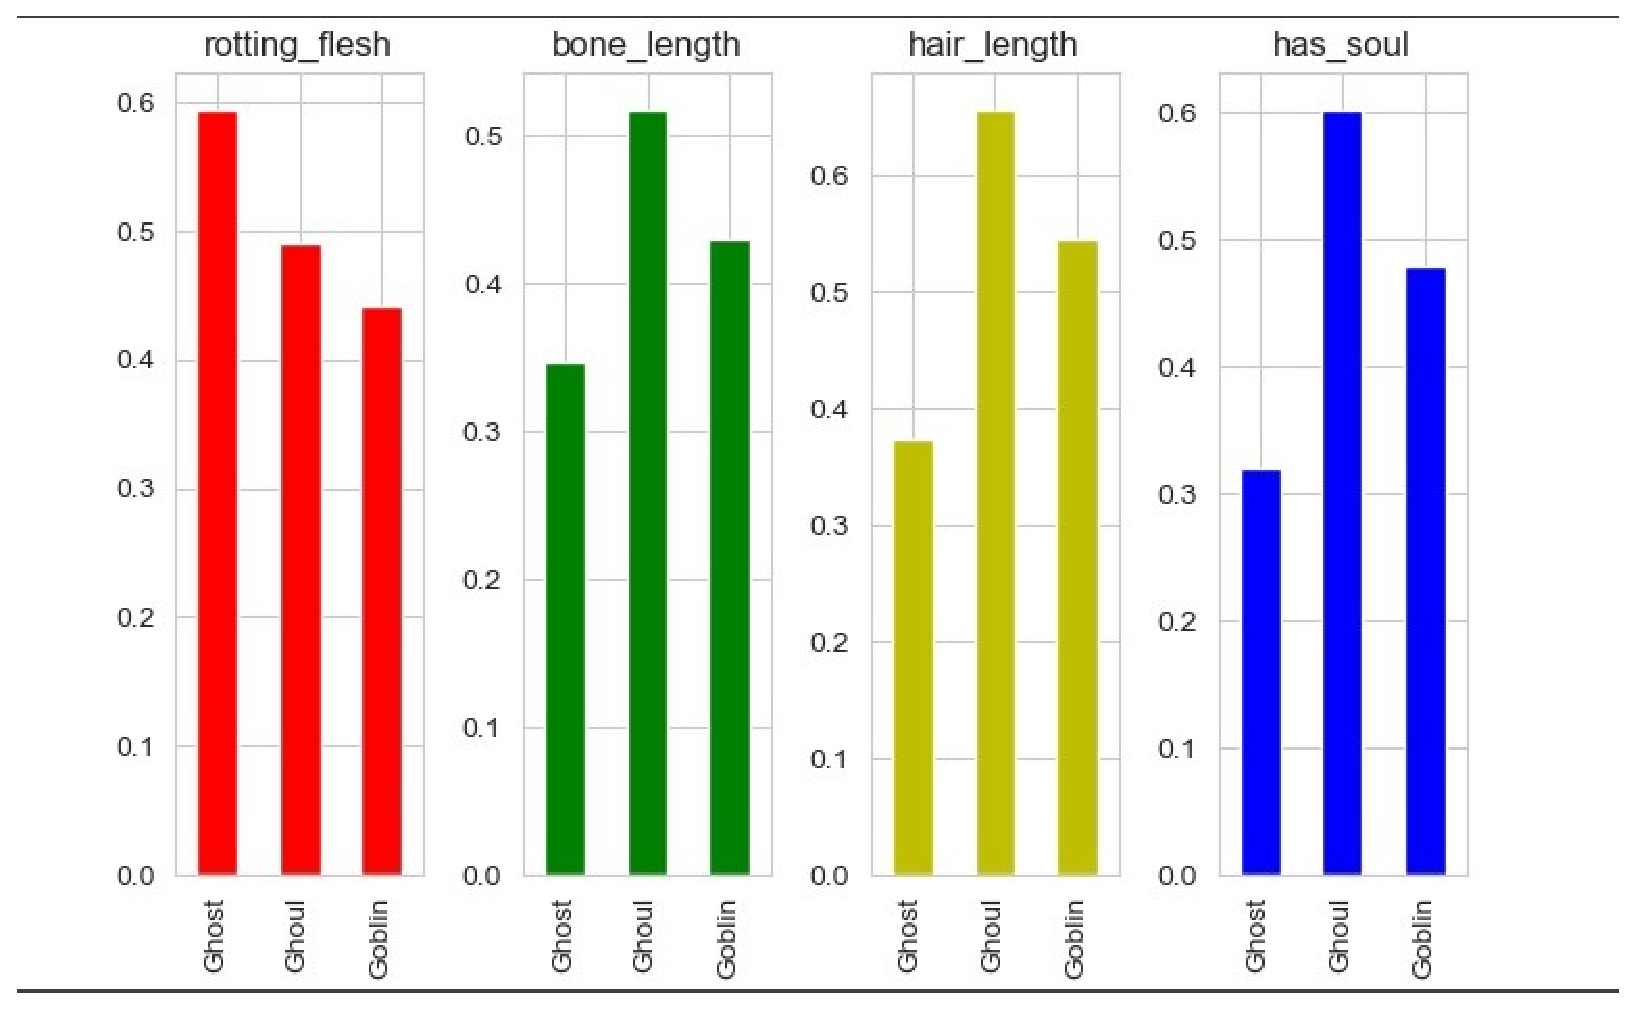
\includegraphics[width=.4\linewidth,height=.4\linewidth]{figures/his_1.eps}
	\end{center}
\end{slide}

\begin{slide}{Data Visualization}
	\begin{center}
		\twotonebox{\rotatebox{90}{Exp}}{\parbox{.96\textwidth}
			{When analyzing the data,
				the boxplot can effectively
				help us identify the characteristics of the data:
				visually identify outliers in the dataset or
				determine the data dispersion and
				bias of the data set.
				We can see that the outliers are very small,
				so can be ignored.
			}}
	\end{center}

	\begin{center}
		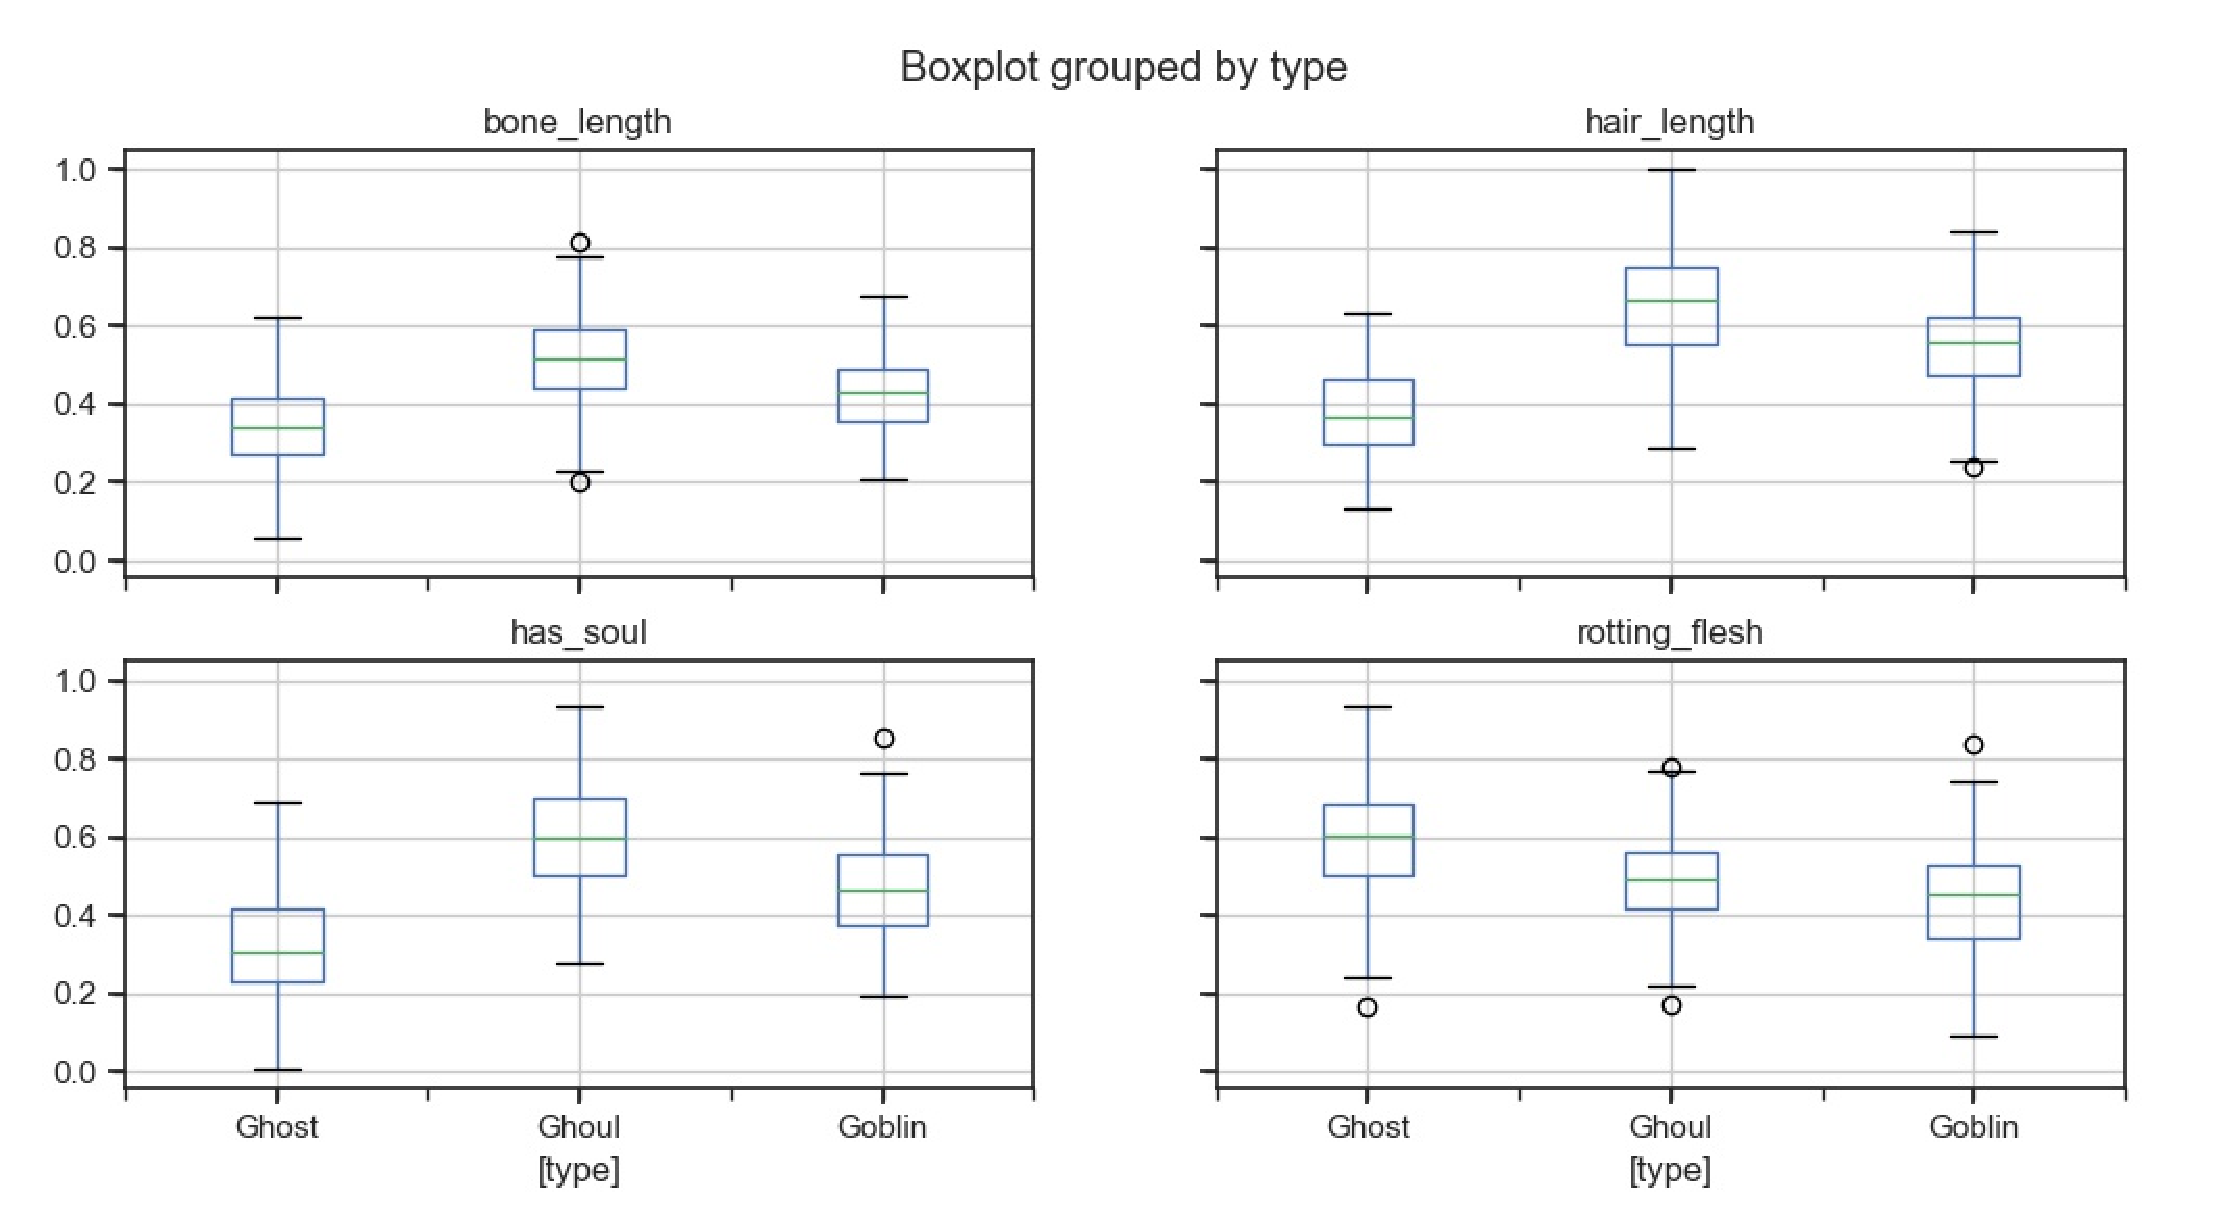
\includegraphics[width=.4\linewidth,height=.4\linewidth]{figures/boxplot.eps}
		\quad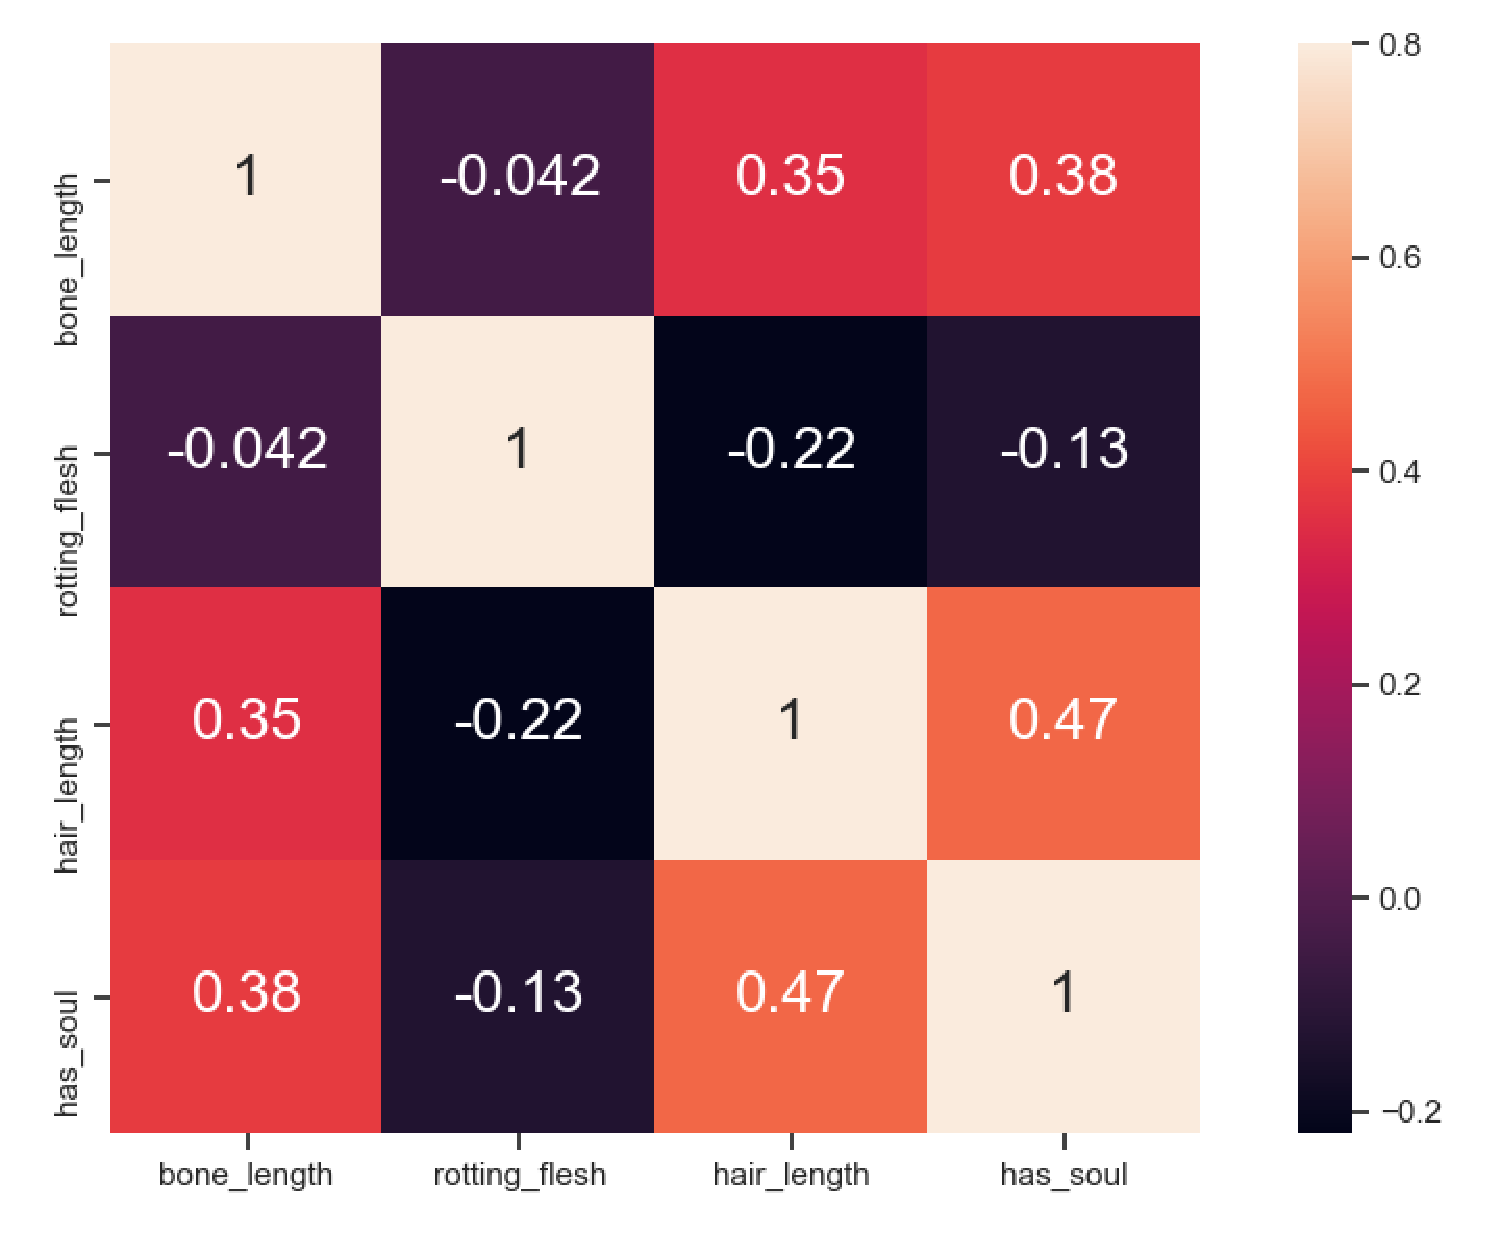
\includegraphics[width=.4\linewidth,height=.4\linewidth]{figures/corr.eps}
	\end{center}
\end{slide}

\begin{slide}{Data Visualization}
	\begin{center}
		\twotonebox{\rotatebox{90}{Exp}}{\parbox{.96\textwidth}
			{It can be seen from the scatter plot that the daily sales volume
				of the product is mainly concentrated between 0 and 1, and the
				price of the product can also be concentrated.
			}}
	\end{center}
	\begin{center}
		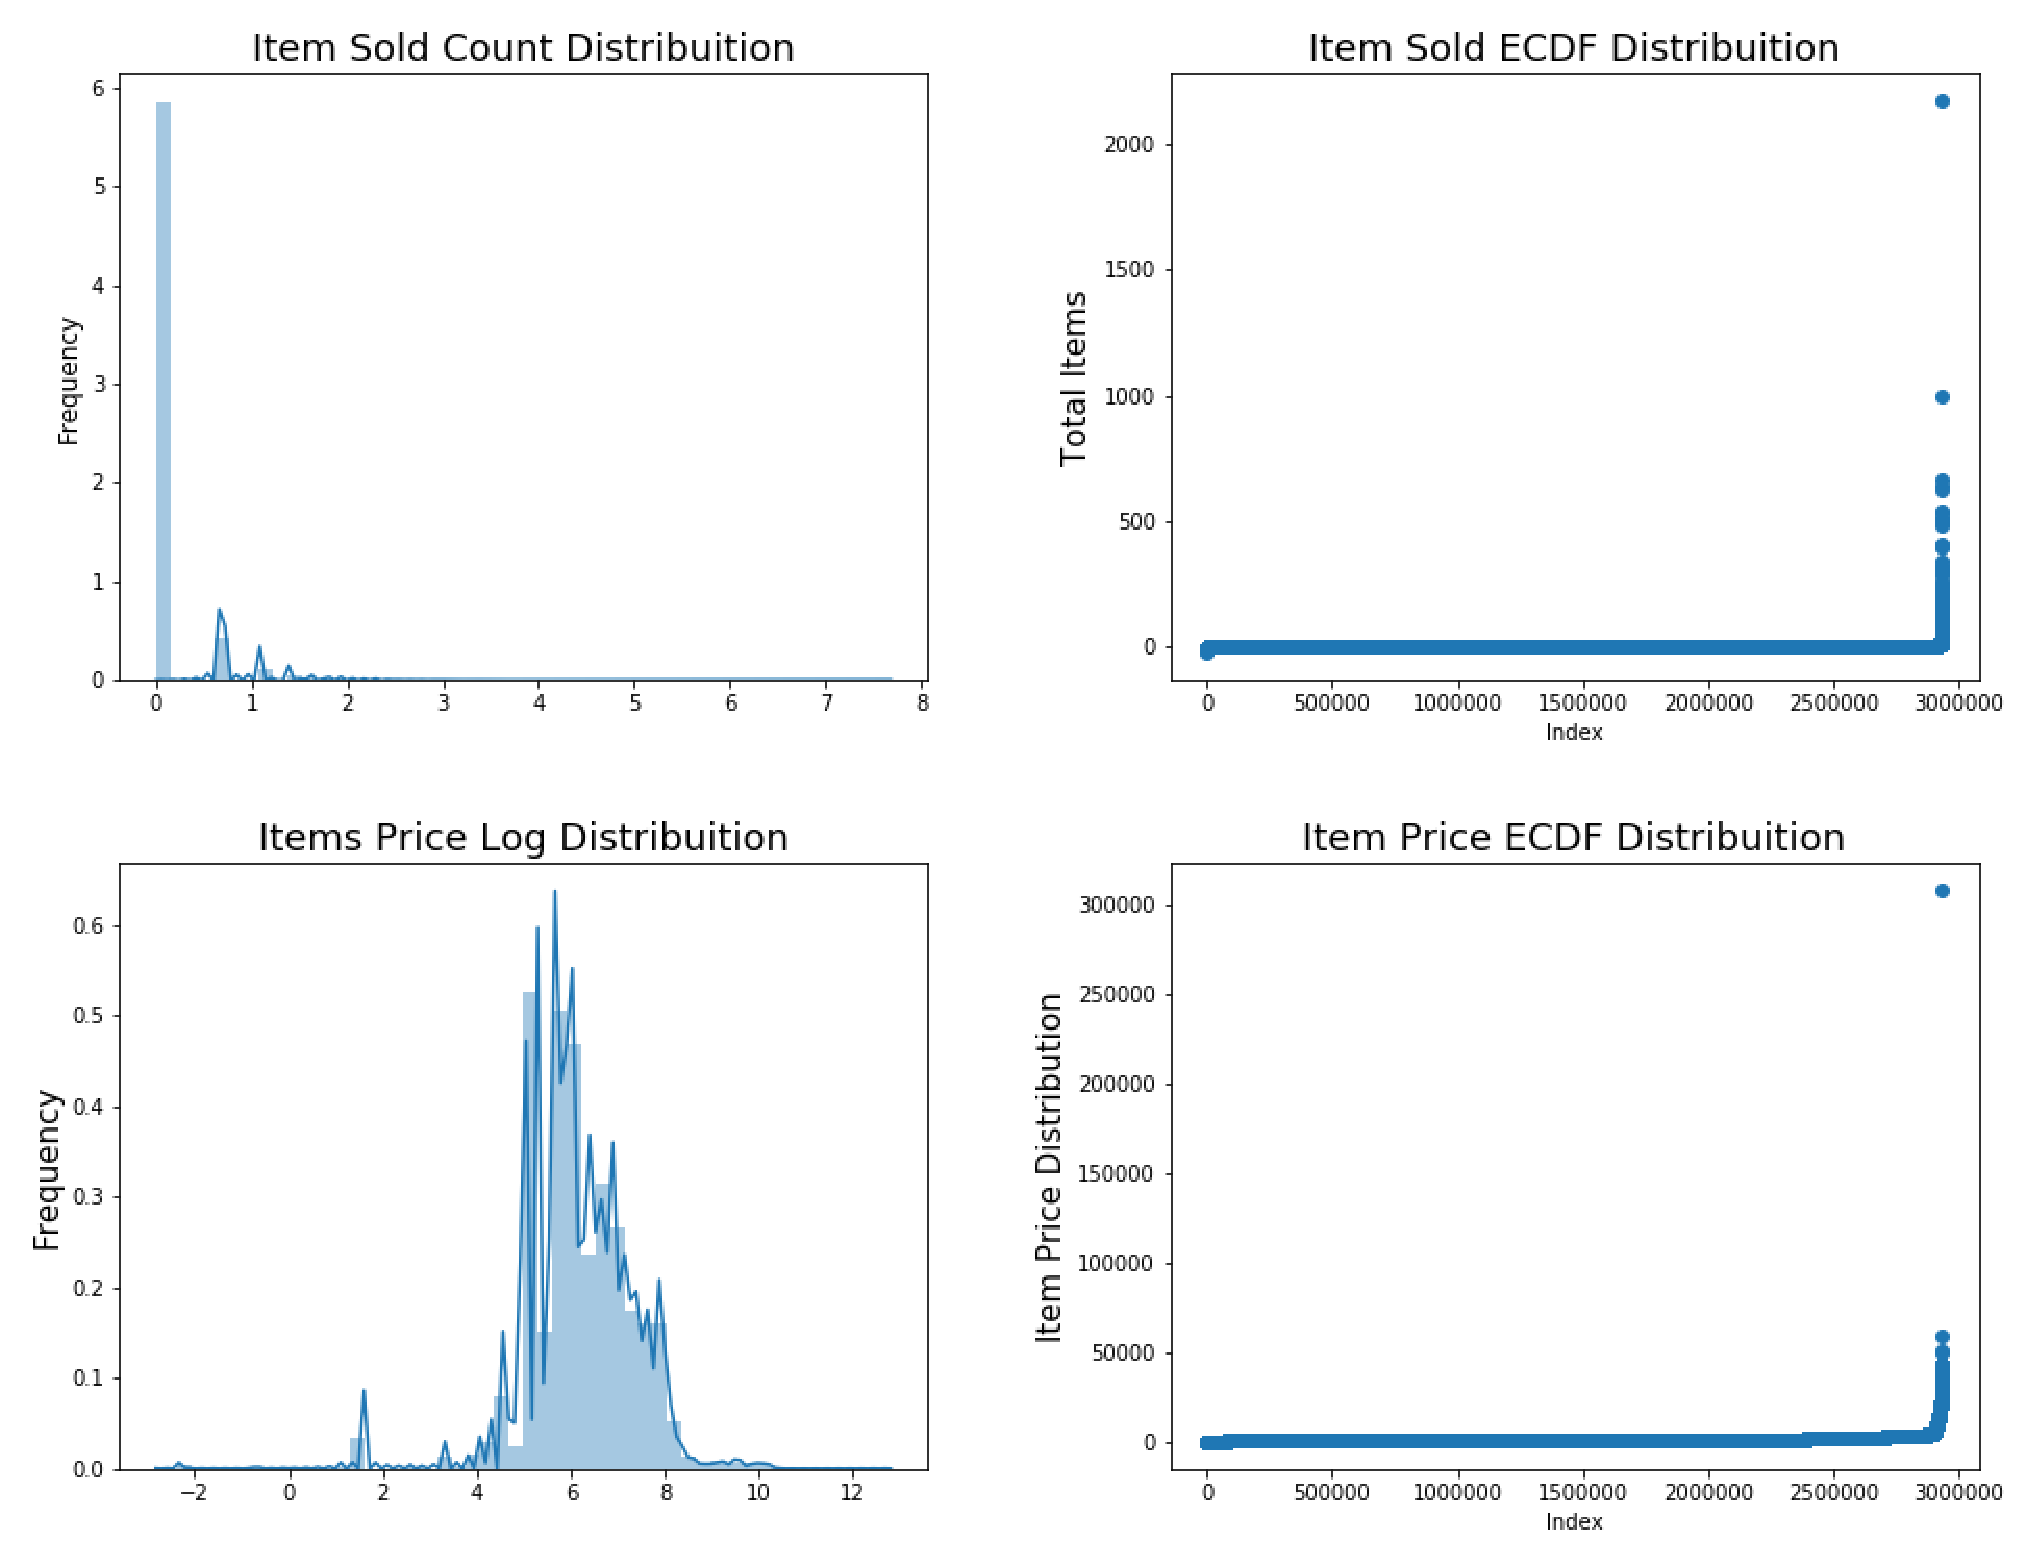
\includegraphics[width=.5\linewidth,height=.4\linewidth]{figures/scatterplot.eps}

	\end{center}
\end{slide}

\section{Feature Engineering}


\begin{slide}{Features importance}

	We take all of these features
	to form a new train datad.

	\begin{center}
		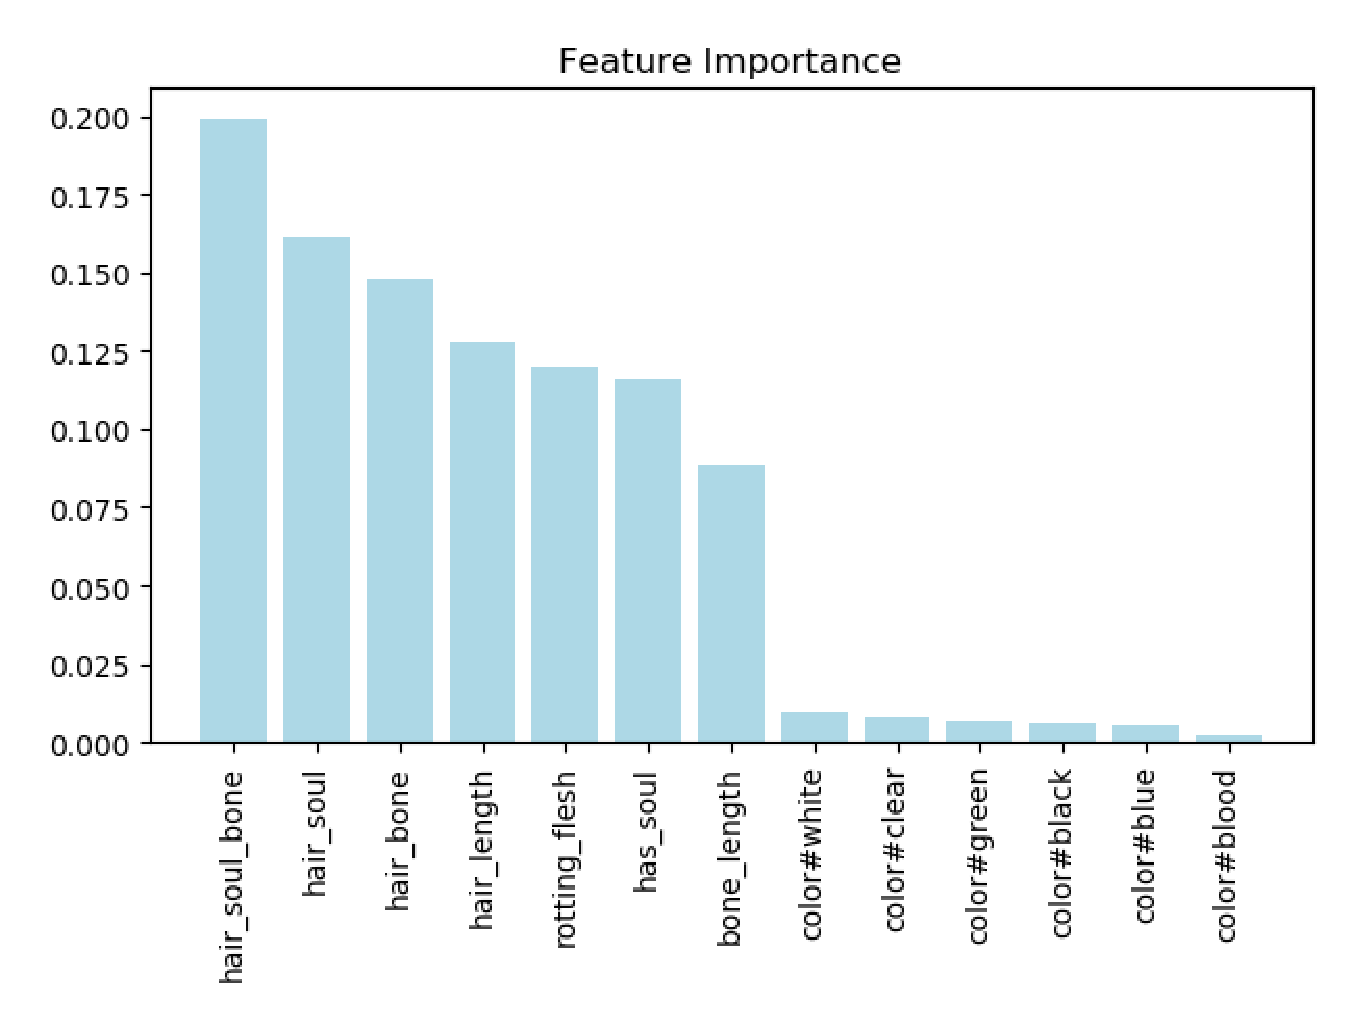
\includegraphics[width=.5\linewidth]{figures/FEATURE.eps}
	\end{center}

\end{slide}

\section{Methods}

\begin{slide}{Ensembling}

	To combine the 1st level model predictions,
	I'll use a simple linear regression.
	As I'm only feeding the model with
	predictions I don't need a complex model.

	\begin{center}
		\begin{itemize}
			\item Base Models
			      \
			      \begin{itemize}
				      \item RandomForest
				      \item XGBoost
				      \item LSTM
				      \item Linear regression
				      \item KNN
			      \end{itemize}
			\item Ensemble Model
			      \
			      \begin{itemize}
				      \item Linear regression
			      \end{itemize}
		\end{itemize}
	\end{center}
\end{slide}

\begin{slide}{Route}

	Here is an image to help the understanding

	\begin{center}
		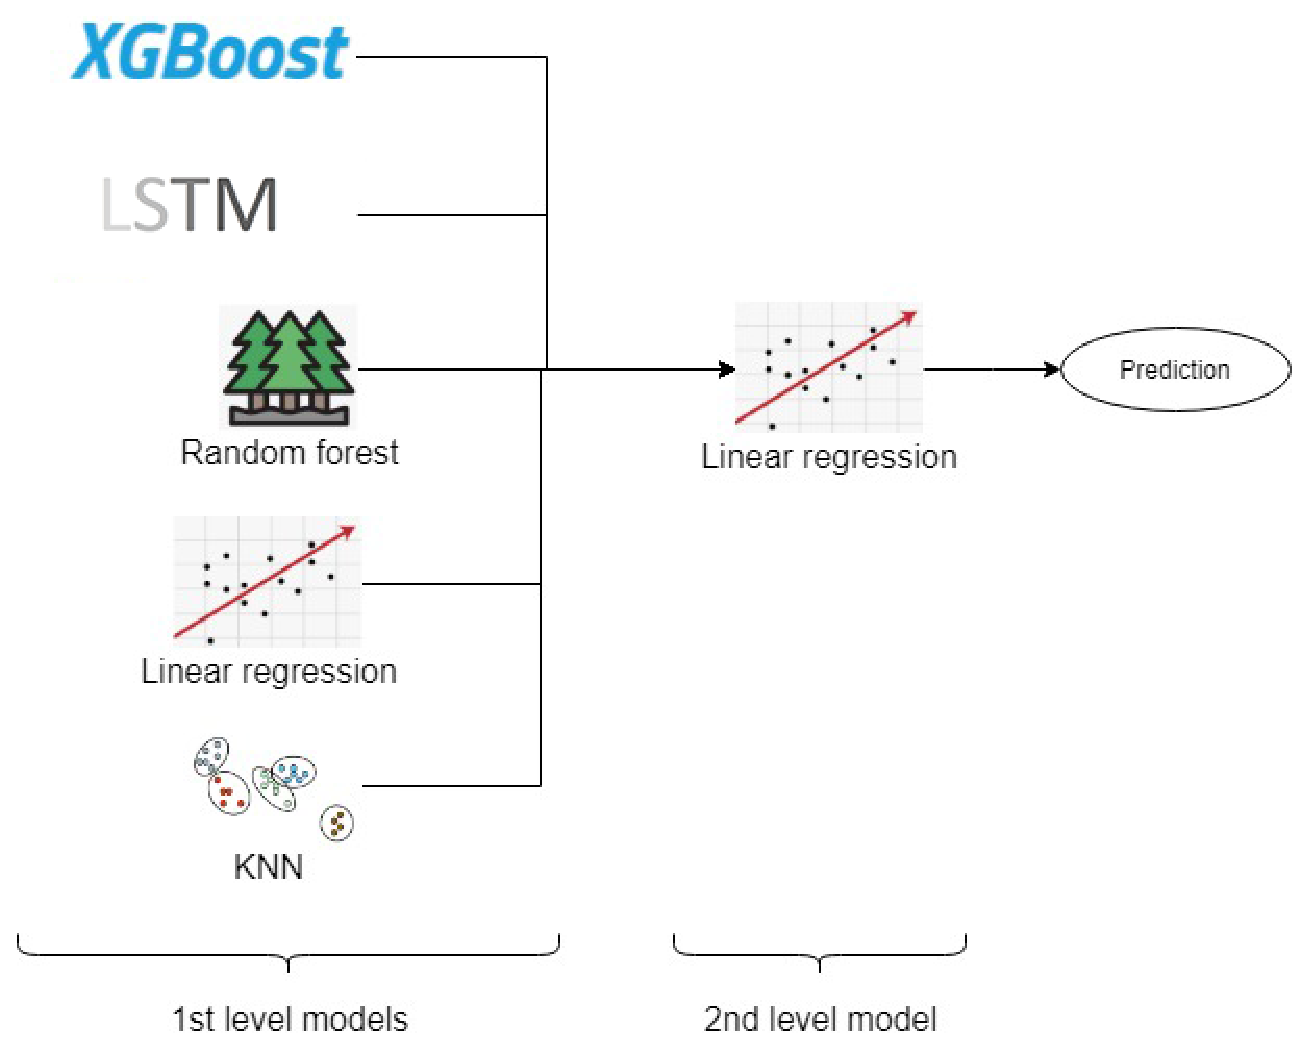
\includegraphics[width=.5\linewidth]{figures/Ensemble.eps}
	\end{center}

\end{slide}

\section{Forecast Results}

\begin{slide}{Evaluation Methods}
	\begin{center}
		\begin{itemize}
			\item RMSE
		\end{itemize}
	\end{center}

\end{slide}
%%==========================================================================================
%%
\begin{slide}{Forecast Results}
	\begin{itemize}
		\item The following are the best Score in training of the base models.
	\end{itemize}
	\begin{center}
		\begin{table}[h]  \centering
			\caption{Best Score of the Base Models}
			\label{tbl:best_score_base_models_old}
			\begin{tabular}{ccccccc}
				%\bottomrule
				\toprule
				                & RandomForest & XGBoost & LSTM   & Linear regression & KNN
				\\
				\midrule
				Train rmse      & 0.8358       & 0.8327  & 0.9276 &
				0.8572          & 0.6976                                                    \\
				Validation rmse & 0.8810       & 0.8959  & 0.6611 &
				0.8806          & 0.8946                                                    \\
				\bottomrule
			\end{tabular}
		\end{table}
	\end{center}
	\begin{itemize}
		\item Ensemble model means using
		      more than 1 model to finish the prediction.
		      The train rmse is 0.764973649571408.
	\end{itemize}

\end{slide}
%%
%%==========================================================================================


%%
%%==========================================================================================


\section{Conclusion}

%%==========================================================================================
%%
\begin{slide}[toc=,bm=]{Conclusion}
	\begin{description}
		\item Exploratory data analysis is
		      very important for the competition,
		      Discover the imperfections of the
		      data and have a certain understanding
		      of the overall appearance of the data,
		      which will help later modeling and analysis.
		\item The data that we have,
		      needed processed in many cases.
		      Data preprocessing includes
		      deal with missing data and outliers,
		      We must think carefully about the outliers,
		      such as ignoring them.
		\item The most important thing is
		      feature engineering.
		      We have to think carefully and
		      deal with outliers, such as ignoring
		      or deleting them.
		\item There is no best model,
		      only the best model. We should
		      try as many models as possible to
		      get the best prediction results.
		\item Feature engineering is very
		      important and even plays a decisive
		      role in this competition.
		\item The Ensemble model may perform better
		      than a single model when dealing
		      with some complex problems.
	\end{description}



\end{slide}

\begin{wideslide}[toc=,bm=]{}
	\centering
	\vspace{\stretch{1}}
	\twocolumn[
		lcolwidth=0.35\linewidth,
		rcolwidth=0.65\linewidth
	]
	{
		% \centerline{\includegraphics[scale=.2]{tulip-logo.eps}}
	}
	{
		\vspace{\stretch{1}}


		\textcolor{black}{\scalebox{2.0}{Thank you \& Question}}


	}
	\vspace{\stretch{1}}
\end{wideslide}

\end{document}
\endinput
